
\فصل{مفاهیم اولیه}

در این فصل به تعریف مفاهیم اولیه و ذکر صورت مسائلی می‌پردازیم که در این پایان‌نامه مورد استفاده قرار گرفته‌اند.

\قسمت{مفاهیم شبکه‌ی عصبی}

\زیرقسمت{تابع فعال‌ساز}

در شبکه‌های عصبی، برای ایجاد خاصیت غیرخطی‌بودن از توابع فعال‌ساز غیرخطی استفاده می‌شود که رابطه‌ی بین ورودی‌های یک گره از شبکه و خروجی آن شبکه را مشخص می‌کند. در این پایان‌نامه مانند مقاله‌ی بلوم و ریوست \مرجع{blum1988training} تابع فعال‌ساز پله را در نظر می‌گیریم که تقریبی از تابع فعال‌ساز سیگماوار\پاورقی{sigmoid} است و به صورت زیر تعریف می‌شود:
\begin{equation*}
	\sigma(x) = \begin{cases}
		0 & x \le 0\\
		1 & x > 0
	\end{cases}
\end{equation*}

\زیرقسمت{شبکه‌ی پرسپترون سه‌لایه}

یک شبکه‌ی پرسپترون چندلایه\پاورقی{multilayer perceptron (MLP)} شامل حداقل سه لایه گره است: یک لایه‌ی ورودی، یک لایه‌ی نهان و یک لایه‌ی خروجی. در چنین شبکه‌ای، گره‌های هر لایه تماماً به گره‌های لایه‌ی قبل و بعد از خود متصل‌اند. شکل~\رجوع{شکل:schematicNN} ساده‌ترین حالت از چنین شبکه‌ای را نشان می‌دهد که در ادامه برای فرمول‌بندی مسئله‌ی تنظیم دقیق  آستانه‌ها استفاده خواهد شد. تابع پله به‌عنوان تابع فعال‌ساز این شبکه انتخاب شده‌است. همان‌طور که در شکل مشاهده می‌شود، به هر نورون علاوه‌بر یال‌های ورودی از لایه‌ی پیشین، یک عدد ثابت به عنوان آستانه یا بایاس\پاورقی{bias} نیز اضافه شده است. مقادیر آستانه همانند وزن‌های یال‌های میان نورون‌ها قابل تنظیم و یادگیری است.

\شروع{شکل}[ht]
\centering
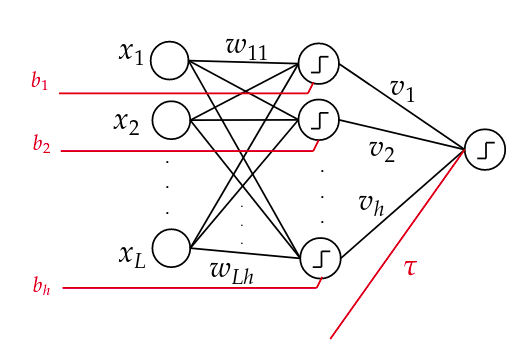
\includegraphics[scale=0.5]{figs/schematicNN.png}
\شرح{شمای شبکه‌ی پرسپترون سه‌لایه. شبکه دارای یک بردار ورودی با بعد $L$، یک خروجی تک‌بعدی دودویی، و یک لایه‌ی نهان با بعد $h$ است.}
\برچسب{شکل:schematicNN}
\پایان{شکل}

اکنون مجموعه داده‌های برچسب‌دار به شکل زوج‌مرتب‌های ورودی-خروجی را در نظر بگیرید که شامل بردارهای ورودی $x^{(j)}$ و برچسب‌های خروجی $y^{(j)}$ است. امتیاز شبکه‌ی فوق روی این مجموعه دادگان\پاورقی{dataset} را به صورت زیر تعریف می‌کنیم، که برابر است با تعداد داده‌هایی که خروجی شبکه با برچسب آن داده برابر است:
\begin{equation} \label{eq:loss}
	score(F, \{(x^{(j)}, y^{(j)})\}) = \sum_{j=1}^N I(F(x^{(j)}) = y^{(j)})
\end{equation}

در این رابطه منظور از $I(\cdot)$ تابع مشخصه‌ای است که مقدار آن در صورت درستی گزاره‌ی ورودی آن برابر با یک، و در غیر اینصورت برابر با صفر است. همچنین $F(\cdot)$ تابعی است که خروجی شبکه‌ی عصبی شکل~\رجوع{شکل:schematicNN} را مشخص می‌کند و می‌توان رابطه‌ی آن را به‌صورت زیر نوشت:
\begin{equation*}
	F(x) = \sigma\left( \tau + \sum_{i=1}^h v_i \sigma(w_i^T x + b_i)\right)
\end{equation*}

هدف از مسئله‌ی یادگیری یا تنظیم دقیق، مقداردهی تمام یا بخشی از یال‌های شبکه است به‌گونه‌ای که امتیاز شبکه روی یک مجموعه دادگان به بیشترین مقدار خود برسد.

\قسمت{مفاهیم الگوریتمی}

\زیرقسمت{مسائل الگوریتمی}

در این بخش به بیان دو مسئله‌ی الگوریتمی می‌پردازیم که در نهایت ارتباط نظری آن‌ها با مسئله‌ی تنظیم دقیق را اثبات خواهیم کرد.

\شروع{تعریف}[جعبه]
یک جعبه در فضای $d$-بعدی که به صورت زیر تعریف می‌شود، مکانی در فضاست که محدود است به ابرصفحه‌هایی موازی با محورهای مختصات:
\begin{equation*}
	<(l_1, l_2, ..., l_d), (r_1, ..., r_d)> := \{(x_1, ..., x_d) ~:~ \forall \ell \in [d] : l_\ell \le x_\ell < r_\ell\}
\end{equation*}
همچنین با مقداردهی $l_i$ با $-\infty$ یا $r_i$ با $+\infty$ می‌توان جعبه‌هایی بی‌کران تعریف کرد. 
\پایان{تعریف}

\شروع{مسئله}[عمق]
تعدادی جعبه در فضای $d$-بعدی داده شده است. یک نقطه‌ی $(p_1, ..., p_d)$ در آن فضا پیدا کنید که متعلق به بیشترین تعداد جعبه‌ها باشد.
\پایان{مسئله}


\شروع{تعریف}[خوشه]
یک خوشه زیرمجموعه‌ای از رأس‌های یک گراف  است که هر دو رأس مجزا از آن به یکدیگر متصل باشند.
\پایان{تعریف}


\شروع{مسئله}[\rl{d}-خوشه]
گرافی با $n$ رأس داده شده است. مشخص کنید که آیا این گراف یک خوشه با حداقل $d$ رأس دارد؟
\پایان{مسئله}

\زیرقسمت{پیچیدگی محاسباتی پارامتری}

نظریه‌ی پیچیدگی محاسباتی به طور سنتی به دنبال تمایز بین مسائلی است که در زمان چندجمله‌ای حل می‌شوند (از طریق یافتن یک الگوریتم کارا) و مسائلی که ان‌پی-سخت‌اند (از طریق یافتن یک کاهش چندجمله‌ای). با این حال دسته‌ی مسائل دوم همچنان طیف وسیعی از مسائل را شامل می‌شوند و نظریاتی برای تمایز بین آن‌ها با ریزدانگی بیشتر پیشنهاد شده‌است. نظریه‌ی پیچیدگی پارامتری یکی از نظریات پیشنهادی است، که پیچیدگی یک مسئله را برحسب پارامتر دیگری از مسئله (افزون بر اندازه‌ی ورودی) بررسی می‌کند. یک دسته از مسائل در این نظریه، دسته‌ی FPT است که توسط داونی و فلوز \مرجع{downey1999parameterized} پیشنهاد شده و به شکل زیر تعریف می‌شود:

\شروع{تعریف}[FPT] مسئله‌ی پارامتری $L \in \Sigma^* \times \mathbb{N}$ یک مسئله‌ی FPT\پاورقی{Fixed-Parameter Tractable} خوانده می‌شود اگر و تنها اگر تابع دلخواه $f(\cdot)$ وجود داشته باشد که بتوان مسئله‌ی $L$ را در زمان
$f(k) \cdot {|x|}^{O(1)}$
حل کرد.
\پایان{تعریف}

مثالی از مسئله‌ای که گمان می‌رود متعلق به دسته‌ی FPT نباشد، مسئله‌ی رنگ‌آمیزی گراف است. می‌دانیم که تشخیص ۳-رنگ‌پذیربودن یک گراف، ان‌پی-کامل است. الگوریتمی از مرتبه‌ی زمانی
$f(k) \cdot {|x|}^{O(1)}$
برای $k=3$ در زمان چندجمله‌ای اجرا خواهد شد. پس اگر مسئله‌ی پارامتری رنگ‌آمیزی گراف در دسته‌ی FPT باشد، آنگاه
$\text{P}=\text{NP}$
نتیجه خواهد شد.

همچنین نامحتمل است که مسئله‌ی پارامتری خوشه که بالاتر تعریف شد متعلق به دسته‌ی FPT باشد. چن و همکاران \مرجع{chen2006strong} نشان داده‌اند که مسئله‌ی خوشه در زمان
$f(k) \cdot n^{o(k)}$
حل نخواهد شد، مگر آنکه حدس ETH\پاورقی{Exponential Time Hypothesis} نقض شود. حدس ETH حدسی قوی‌تر از
$\text{P} \neq \text{NP}$
است که بیان می‌کند مسئله‌ی ۳-صدق‌پذیری\پاورقی{3-SAT} در زمان کمتر از نمایی یعنی در زمان $2^{o(n)}$ حل نمی‌شود.

برای آنکه نشان دهیم مسئله‌ی جدیدی دارای درجه‌ی سختی پارامتری مشابه با مسئله‌ی خوشه است و در نتیجه به احتمال بالا متعلق به دسته‌ی FPT نیست، نیاز است که یک کاهش FPT از مسئله‌ی خوشه به آن مسئله ارائه دهیم. مطابق \مرجع{downey1999parameterized} چنین کاهشی به صورت زیر تعریف می‌شود:

\شروع{تعریف}[کاهش \rl{FPT}]
یک کاهش FPT از مسئله‌ی $P$ به مسئله‌ی $Q$، تابع $\phi$ با شرایط زیر است:

\شروع{فقرات}
\فقره $\phi(x)$ یک نمونه‌ی مثبت\پاورقی{yes-instance} برای مسئله‌ی $Q$ است اگر و تنها اگر $x$ یک نمونه‌ی مثبت برای مسئله‌ی $P$ باشد.
\فقره $\phi(x)$ قابل محاسبه در زمان
$f(k) \cdot {|x|}^{O(1)}$
باشد، که $k$ همان پارامتر برای ورودی $x$ است.
\فقره اگر $k$ پارامتر ورودی $x$ و $k'$ پارامتر ورودی $\phi(x)$ باشد، تابع $g$ وجود داشته باشد که $k' \leq g(k)$ باشد.
\پایان{فقرات}

\پایان{تعریف}

در فصل ۴ یک کاهش FPT از مسئله‌ی خوشه به مسئله‌ی تنظیم دقیق آستانه‌ها ارائه خواهیم کرد که نشان خواهد داد مسئله‌ی دوم نیز متعلق به دسته‌ی FPT نیست و نامحتمل است که در زمان
$f(k) \cdot n^{o(k)}$
حل شود.


%%%%%%%%%%%%%%%%%%%%%%%%%%%%%%%%%%%%%%%%%%%%%%%%%%

\begin{comment}
\قسمت{نحوه‌ی نگارش}

\زیرقسمت{پرونده‌ها}

پرونده‌ی اصلی پایان‌نامه در قالب استاندارد\زیرنویس{
قالب استاندارد از گیت‌هاب به نشانی
\href{https://github.com/zarrabi/thesis-template}
{github.com/zarrabi/thesis-template}
قابل دریافت است.}
\کد{thesis.tex}  نام دارد.
به ازای هر فصل از پایان‌نامه، یک پرونده در شاخه‌ی \کد{chapters} ایجاد نموده
و نام آن را در  \کد{thesis.tex} (در قسمت فصل‌ها) درج نمایید.
برای مشاهده‌ی خروجی، پرونده‌ی \کد{thesis.tex} را با زی‌لاتک کامپایل کنید.
مشخصات اصلی پایان‌نامه را می‌توانید در پرونده‌ی \کد{front/info.tex} ویرایش کنید.

\زیرقسمت{عبارات ریاضی}

برای درج عبارات ریاضی در داخل متن از \$...\$ و 
برای درج عبارات ریاضی در یک خط مجزا از \$\$...\$\$ یا محیط \لر{equation} 
استفاده کنید. برای مثال عبارت 
$2x + 3y$
در داخل متن و عبارت زیر
\begin{equation}
\sum_{k=0}^{n} {n \choose k} = 2^n
\end{equation}
در یک خط مجزا درج شده است. 
دقت کنید که تمامی عبارات ریاضی، از جمله متغیرهای تک‌حرفی مانند $x$ و $y$ باید در محیط ریاضی 
یعنی محصور بین دو علامت \$ باشند. 


\زیرقسمت{علائم ریاضی پرکاربرد}

برخی علائم ریاضی پرکاربرد در زیر فهرست شده‌اند. 
برای مشاهده‌ی دستور  معادل پرونده‌ی منبع را ببینید.


\شروع{فقرات}
\فقره مجموعه‌‌های اعداد: 
$\IN, \IZ, \IZ^+, \IQ, \IR, \IC$
\فقره مجموعه:
$\set{1, 2, 3}$
\فقره دنباله‌:
$\seq{1, 2, 3}$
\فقره سقف و کف:
$\ceil{x}, \floor{x}$
\فقره اندازه و متمم:
$\card{A}, \setcomp{A}$
\فقره همنهشتی:
$a \iequiv{n} 1$
یا
$a \equiv 1 \imod{n}$ 
%\فقره شمردن (عاد کردن):
%$3 \divs n, 2 \ndivs n$
\فقره ضرب و تقسیم:
$\times, \cdot, \div$
\فقره سه‌نقطه‌:
$1, 2, \dots, n$
\فقره کسر و ترکیب:
${n \over k}, {n \choose k}$
\فقره اجتماع و اشتراک:
$A \cup (B \cap C)$
\فقره عملگرهای منطقی:
$\neg p \vee (q \wedge r)$

\فقره پیکان‌ها:
$\rightarrow, \Rightarrow, \leftarrow, \Leftarrow, \leftrightarrow, \Leftrightarrow$
\فقره عملگرهای مقایسه‌ای:
$\not=, \le, \not\le, \ge, \not\ge$
\فقره عملگرهای مجموعه‌ای:
$\in, \not\in, \setminus, \subset, \subseteq, \subsetneq, \supset, \supseteq, \supsetneq$

\فقره جمع و ضرب چندتایی:
$\sum_{i=1}^{n} a_i, \prod_{i=1}^{n} a_i$
\فقره اجتماع و اشتراک چندتایی:
$\bigcup_{i=1}^{n} A_i, \bigcap_{i=1}^{n} A_i$
\فقره برخی نمادها:
$\infty, \emptyset, \forall, \exists, \triangle, \angle, \ell, \equiv, \therefore$
\پایان{فقرات}


\زیرقسمت{لیست‌ها}

برای ایجاد یک لیست‌ می‌توانید از محیط‌های «فقرات» و «شمارش» همانند زیر استفاده کنید.

\begin{multicols}{2}
\شروع{فقرات}
\فقره مورد اول
\فقره مورد دوم
\فقره مورد سوم
\پایان{فقرات}

\شروع{شمارش}
\فقره مورد اول
\فقره مورد دوم
\فقره مورد سوم
\پایان{شمارش}

\end{multicols}


\زیرقسمت{درج شکل}

یکی از روش‌های مناسب برای ایجاد شکل استفاده از نرم‌افزار \لر{LaTeX Draw} و سپس
درج خروجی آن به صورت یک فایل \کد{tex} درون متن 
با استفاده از دستور  \کد{fig} یا \کد{centerfig} است.
شکل~\رجوع{شکل:پوشش رأسی} نمونه‌ای از اشکال ایجادشده با این ابزار را نشان می‌دهد.


\شروع{شکل}[ht]
\centerfig{cover.tex}{.9}
\شرح{یک گراف و پوشش رأسی آن}
\برچسب{شکل:پوشش رأسی}
\پایان{شکل}

\bigskip
همچنین می‌توانید با استفاده از نرم‌افزار \lr{Ipe} شکل‌های خود را مستقیما
به صورت \لر{pdf} ایجاد نموده و آن‌ها را با دستورات \کد{img} یا  \کد{centerimg} 
درون متن درج کنید. برای نمونه، شکل~\رجوع{شکل:گراف جهت‌دار} را ببینید.


\شروع{شکل}[ht]
\centerimg{strip}{6.5cm}
\شرح{نمونه شکل ایجادشده توسط نرم‌افزار \lr{Ipe}}
\برچسب{شکل:گراف جهت‌دار}
\پایان{شکل}


\زیرقسمت{درج جدول}

برای درج جدول می‌توانید با استفاده از دستور  «جدول»
جدول را ایجاد کرده و سپس با دستور  «لوح»  آن را درون متن درج کنید.
برای نمونه جدول~\رجوع{جدول:عملگرهای مقایسه‌ای} را ببینید.

\vspace{1.5em}

\شروع{لوح}[ht]
\تنظیم‌ازوسط
\شرح{عملگرهای مقایسه‌ای}

\شروع{جدول}{|c|c|}
\خط‌پر 
\سیاه عملگر & \سیاه عنوان \\ 
\خط‌پر \خط‌پر 
\کد{<} & کوچک‌تر \\ 
\کد{>} & بزرگ‌تر \\
\کد{==} &  مساوی \\ 
\کد{<>} & نامساوی \\ 
\خط‌پر
\پایان{جدول}

\برچسب{جدول:عملگرهای مقایسه‌ای}
\پایان{لوح}



\زیرقسمت{درج الگوریتم}

برای درج الگوریتم می‌توانید از محیط «الگوریتم» استفاده کنید.
یک نمونه در الگوریتم~\رجوع{الگوریتم: پوشش رأسی حریصانه} آمده است.

\شروع{الگوریتم}{پوشش رأسی حریصانه}
\ورودی گراف $G=(V, E)$
\خروجی یک پوشش رأسی از $G$

\دستور قرار بده $C = \emptyset$  % \توضیحات{مقداردهی اولیه}
\تاوقتی{$E$ تهی نیست}
%\اگر{$|E| > 0$}
%	\دستور{یک کاری انجام بده}
%\پایان‌اگر
\دستور یال دل‌‌خواه $uv \in E$ را انتخاب کن
\دستور رأس‌های $u$ و $v$ را به $C$ اضافه کن
\دستور تمام یال‌های واقع بر $u$ یا $v$ را از $E$ حذف کن
\پایان‌تاوقتی
\دستور $C$ را برگردان
\پایان{الگوریتم}


\زیرقسمت{محیط‌های ویژه}

برای درج مثال‌ها، قضیه‌ها، لم‌ها و نتیجه‌ها به ترتیب از محیط‌های
«مثال»، «قضیه»، «لم» و «نتیجه» استفاده کنید.
برای درج اثبات قضیه‌ها و لم‌ها  از محیط «اثبات» استفاده کنید.

تعریف‌های داخل متن را با استفاده از دستور «مهم» به صورت \مهم{تیره‌} نشان دهید.
تعریف‌های پایه‌ای‌تر را درون محیط «تعریف» قرار دهید.

\شروع{تعریف}[اصل لانه‌کبوتری]
اگر $n+1$ کبوتر یا بیش‌تر درون  $n$ لانه قرار گیرند، آن‌گاه لانه‌ای 
وجود دارد که شامل حداقل دو کبوتر است.
\پایان{تعریف}




\قسمت{برخی نکات نگارشی}

این فصل حاوی برخی نکات ابتدایی ولی بسیار مهم در نگارش متون فارسی است. 
نکات گردآوری‌شده در این فصل به‌ هیچ‌ وجه کامل نیست، 
ولی دربردارنده‌ی حداقل مواردی است که رعایت آن‌ها در نگارش پایان‌نامه ضروری به نظر می‌رسد.

\زیرقسمت{فاصله‌گذاری}

\شروع{شمارش}

\فقره 
علائم سجاوندی مانند نقطه، ویرگول، دونقطه، نقطه‌ویرگول، علامت سؤال و علامت تعجب % (. ، : ؛ ؟ !) 
بدون فاصله از کلمه‌ی پیشین خود نوشته می‌شوند، ولی بعد از آن‌ها باید یک فاصله‌ قرار گیرد. مانند: من، تو، او.
\فقره 
علامت‌های پرانتز، آکولاد، کروشه، نقل قول و نظایر آن‌ها بدون فاصله با عبارات داخل خود نوشته می‌شوند، ولی با عبارات اطراف خود یک فاصله دارند. مانند: (این عبارت) یا \{آن عبارت\}.
\فقره 
دو کلمه‌ی متوالی در یک جمله همواره با یک فاصله از هم جدا می‌شوند، ولی اجزای یک کلمه‌ی مرکب باید با نیم‌فاصله\زیرنویس{«نیم‌فاصله» فاصله‌‌ای مجازی است که در عین جدا کردن اجزای یک کلمه‌ی مرکب از یک‌دیگر، آن‌ها را نزدیک به هم نگه می‌دارد. معمولاً برای تولید این نوع فاصله در صفحه‌کلید‌های استاندارد از ترکیب Shift+Space استفاده می‌شود.}‌‌
 از هم جدا شوند. مانند: کتاب درس، محبت‌آمیز، دوبخشی.
 \فقره 
 اجزای فعل‌های مرکب با فاصله از یک‌دیگر نوشته می‌شوند، مانند: تحریر کردن، به سر آمدن.
\پایان{شمارش}


\زیرقسمت{شکل حروف}

\شروع{شمارش}

\فقره 
در متون فارسی به جای حروف «ك» و «ي» عربی باید از حروف «ک» و «ی» فارسی استفاده شود. همچنین به جای اعداد عربی مانند ٥ و ٦ باید از اعداد فارسی مانند ۵ و ۶ استفاده نمود. 
برای این کار، توصیه می‌شود صفحه‌کلید‌ فارسی استاندارد\زیرنویس{\href{http://persian-computing.ir/download/Iranian_Standard_Persian_Keyboard_(ISIRI_9147)_(Version_2.0).zip}{صفحه‌کلید فارسی استاندارد برای ویندوز}، تهیه‌شده توسط بهنام اسفهبد} را بر روی سیستم خود نصب کنید.
\فقره 
عبارات نقل‌قول‌شده یا مؤکد باید درون علامت نقل قولِ «» قرار گیرند، نه ''``. مانند: «کشور ایران».
\فقره 
کسره‌ی اضافه‌ی بعد از «ه» غیرملفوظ به صورت «ه‌ی» یا «هٔ» نوشته می‌شود. مانند: خانه‌ی علی، دنباله‌ی فیبوناچی.

        تبصره‌: اگر «ه» ملفوظ باشد، نیاز به «‌ی» ندارد. مانند: فرمانده دلیر، پادشه خوبان. 

\فقره 
پایه‌های همزه در کلمات، همیشه «ئـ» است، مانند: مسئله و مسئول، مگر در مواردی که همزه ساکن است که در این ‌صورت باید متناسب با اعراب حرف پیش از خود نوشته شود. مانند: رأس، مؤمن. 

\پایان{شمارش}


\زیرقسمت{جدانویسی}

\شروع{شمارش}


\فقره 
علامت استمرار، «می»، توسط نیم‌فاصله از جزء‌ بعدی فعل جدا می‌شود. مانند: می‌رود، می‌توانیم.
\فقره 
شناسه‌های «ام»، «ای»، «ایم»، «اید» و «اند» توسط نیم‌فاصله، و شناسه‌ی «است» توسط فاصله از کلمه‌ی پیش از خود جدا می‌شوند. مانند: گفته‌ام، گفته‌ای، گفته است.
\فقره 
علامت جمع «ها» توسط نیم‌فاصله از کلمه‌ی پیش از خود جدا می‌شود. مانند: این‌ها، کتاب‌ها.
\فقره 
«به» همیشه جدا از کلمه‌ی بعد از خود نوشته می‌شود، مانند: به‌ نام و به آن‌ها، مگر در مواردی که «بـ» صفت یا فعل ساخته است. مانند: بسزا، ببینم.
\فقره 
«به» همواره با فاصله از کلمه‌ی بعد از خود نوشته می‌شود، مگر در مواردی که «به» جزئی از یک اسم یا صفت مرکب است. مانند: تناظر یک‌به‌یک، سفر به تاریخ. 
%\پایان{شمارش}
%
%
%\زیرقسمت{جدانویسی مرجح}
%
%\شروع{شمارش}

%\فقره 
%اجزای اسم‌ها، صفت‌ها، و قیدهای مرکب توسط نیم‌فاصله از یک‌دیگر جدا می‌شوند. مانند: دانش‌جو، کتاب‌خانه، گفت‌وگو، آن‌گاه، دل‌پذیر.
%
%        تبصره: اجزای منتهی به «هاء ملفوظ» را می‌توان از این قانون مستثنی کرد. مانند: راهنما، رهبر. 

\فقره 
علامت صفت برتری، «تر»، و علامت صفت برترین، «ترین»، توسط نیم‌فاصله از کلمه‌ی پیش از خود جدا می‌شوند. 
مانند: سنگین‌تر، مهم‌ترین.

        تبصره‌: کلمات «بهتر» و «بهترین» را می‌توان از این قاعده مستثنی نمود. 

\فقره 
پیشوندها و پسوندهای جامد، چسبیده به کلمه‌ی پیش یا پس از خود نوشته می‌شوند. مانند: همسر، دانشکده، دانشگاه.

        تبصره‌: در مواردی که خواندن کلمه دچار اشکال می‌شود، می‌توان پسوند یا پیشوند را جدا کرد. مانند: هم‌میهن، هم‌ارزی. 

\فقره 
ضمیرهای متصل چسبیده به کلمه‌ی پیش‌ از خود نوشته می‌شوند. مانند: کتابم، نامت، کلامشان. 

\پایان{شمارش}

\end{comment}

